\chapter{Modellazione dei Casi d'Uso}
\section{Attori e Casi d'Uso}
\begin{table}[!hbp]
	\centering
	\begin{tblr}{colspec=XX}
		\begin{minipage}[t]{\linewidth}
			\paragraph{Attori primari}
			\begin{itemize}
				\item UtenteNonRegistrato
				\item UtenteRegistrato
				\item Utente
				\item Amministratore
			\end{itemize}
		\end{minipage} &
		\begin{minipage}[t]{\linewidth}
			\paragraph{Attori secondari}
			\begin{itemize}
				\item SistemaGestioneAcquisti	
			\end{itemize}
		\end{minipage} \\
	\end{tblr}
\end{table}
\begin{table}[!hbp]
	\centering
	\begin{tblr}{colspec=XX}
		\begin{minipage}[t]{\linewidth}
			\paragraph{Casi d'uso}
			\begin{enumerate}
				\item Registrazione 
				\item Autenticazione
				\item RicercaEvento
				\item PubblicaEvento
				\item ConsultaInfromazioniEvento
				\item ConsultaCatalogoEventi
				\item PartecipazioneEvento
				\item AcquistoBiglietto
				\item ModificaDatiPersonali
				\item ConsultaStoricoBiglietti
				\item VisualizzaBiglietto
				\item ScaricaBiglietto
			\end{enumerate}
		\end{minipage} &
		\begin{minipage}[t]{\linewidth}
			\paragraph{Casi d'uso di inclusione}
			\begin{enumerate}
                \item ConsultaCatalogoEventi
			\end{enumerate}

		\end{minipage}
	\end{tblr}
\end{table}
\begin{table}[!ht]
\centering
\small
\begin{tblr}{
  colspec = {X[2,l] X[1.2,l] X[1.7,l] X[1.6,l] X[1.5,l]},
  hlines,
  row{1} = {font=\bfseries}
}
Caso d'uso & Attori Primari & Attori Secondari & Incl. / Ext. & Requisiti corrispondenti \\
Registrazione & UtenteNonRegistrato & -- & -- & \Req{rf}{01} \\
Aunteticazione & UtenteRegistrato & -- & -- & \Req{rf}{02} \\
RicercaEvento & UtenteRegistrato & -- & -- &\Req{rf}{08} \\
PubblicaEvento & Amministratore & -- & -- & \Req{rf}{06} \\
ConsultaInformazioniEvento & Amministratore & -- & Include: Consulta Catalogo Eventi & \Req{rf}{16}, \Req{rf}{17} \\
ConsultaCatalogoEventi & UtenteRegistrato & --  & -- & \Req{rf}{07} \\
PartecipazioneEvento& Utente & -- & -- & \Req{rf}{14} \\
AcquistaBiglietto & Utente & SistemaGestioneAcquisti & Include: ConsultaCatalogoEventi & \Req{rf}{09} \\
ModificaDatiPersonali & Utente & -- & -- & \Req{rf}{5} \\
ConsultaStoricoBiglietti & Utente & -- & --  & \Req{rf}{04} \\
VisualizzaBiglietto & Utente & -- & -- & \Req{rf}{11} \\
ScaricaBiglietto & Utente & -- & -- & \Req{rf}{12} \\
\end{tblr}
\end{table}

\section{Diagramma dei Casi d'Uso}
\begin{table}[!ht]
\centering
	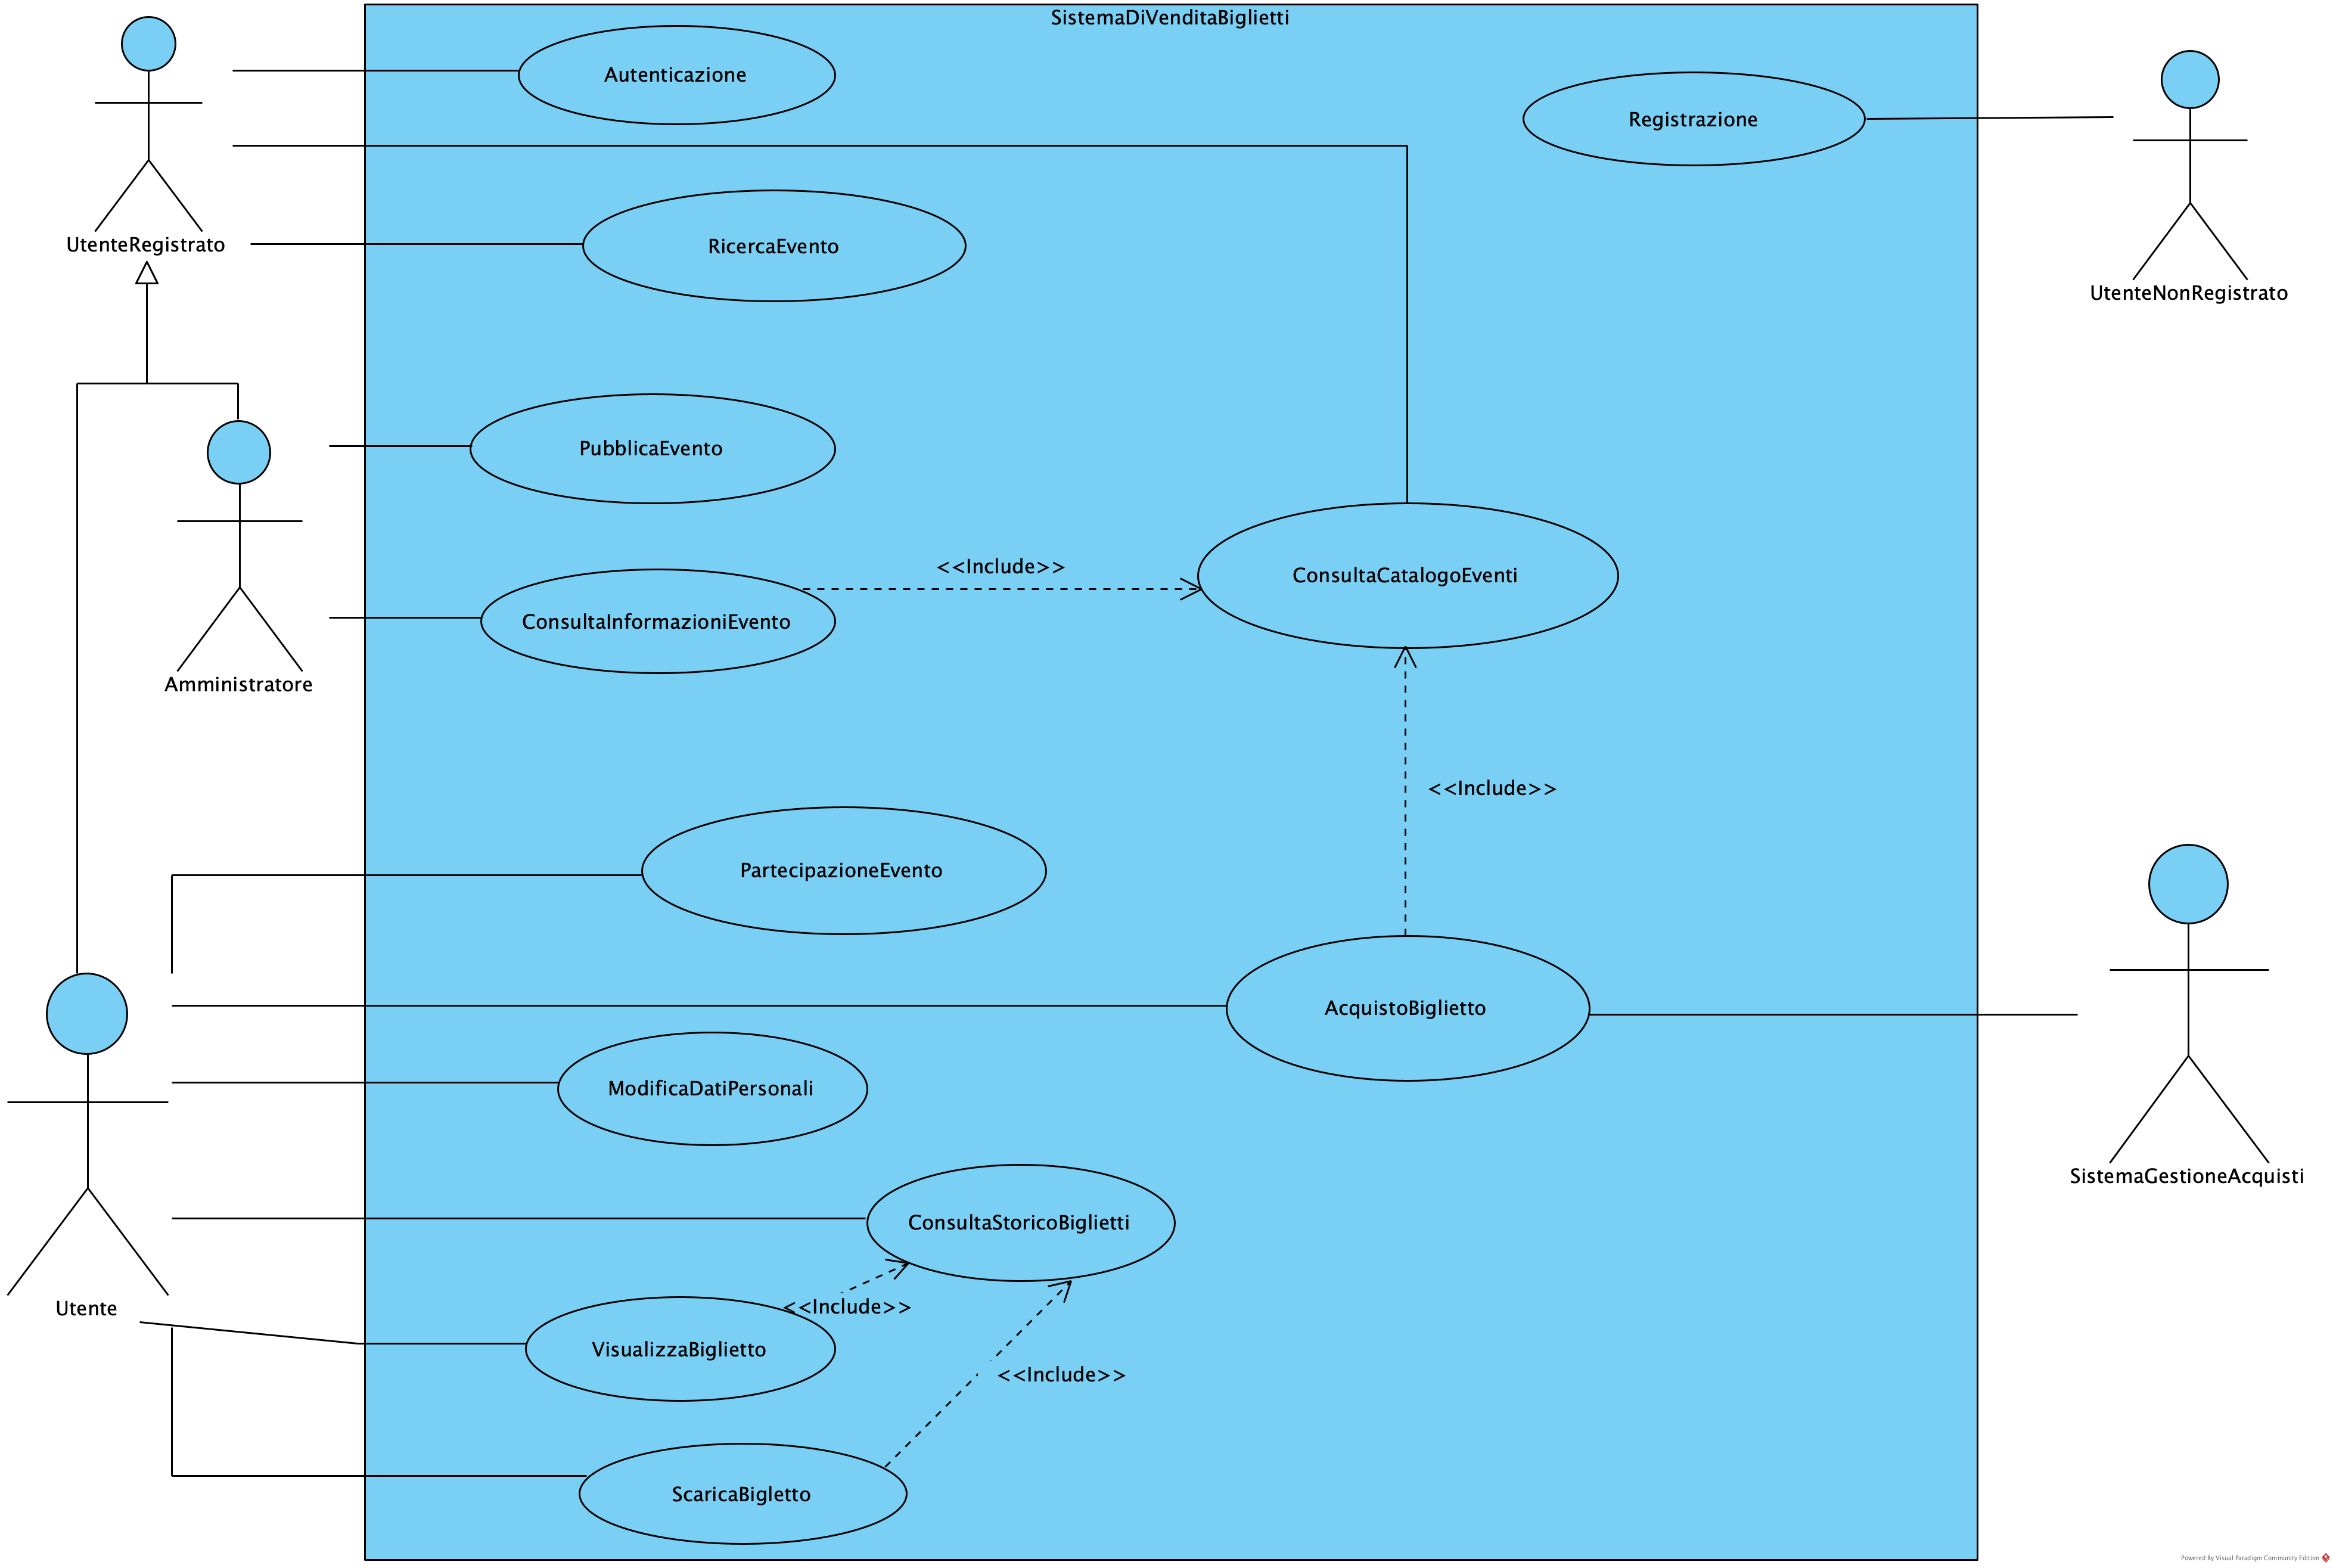
\includegraphics[width=\linewidth]{assets/casid'uso/usd.png}
\end{table}	
\pagebreak
\section{Scenari}
\IncludeTable{capitoli/scenari/Registrazione}
\IncludeTable{capitoli/scenari/Autenticazione}
\IncludeTable{capitoli/scenari/ModificaDatiPersonali}
\IncludeTable{capitoli/scenari/RichiediCatalogoEventi}
\IncludeTable{capitoli/scenari/RicercaEvento}
\IncludeTable{capitoli/scenari/VisualizzaBiglietto}
\IncludeTable{capitoli/scenari/ConsultaStoricoBiglietti}
\IncludeTable{capitoli/scenari/ScaricaBiglietto}
\IncludeTable{capitoli/scenari/AcquistaBiglietto}
\IncludeTable{capitoli/scenari/PubblicaEvento}
\IncludeTable{capitoli/scenari/PartecipazioneEvento}
\IncludeTable{capitoli/scenari/ConsultaInformazioniEvento}
\newpage
\section{Diagramma delle Classi}
Di seguito riportiamo il diagramma delle classi di analisi.
\begin{figure}[!ht]
	\centering
	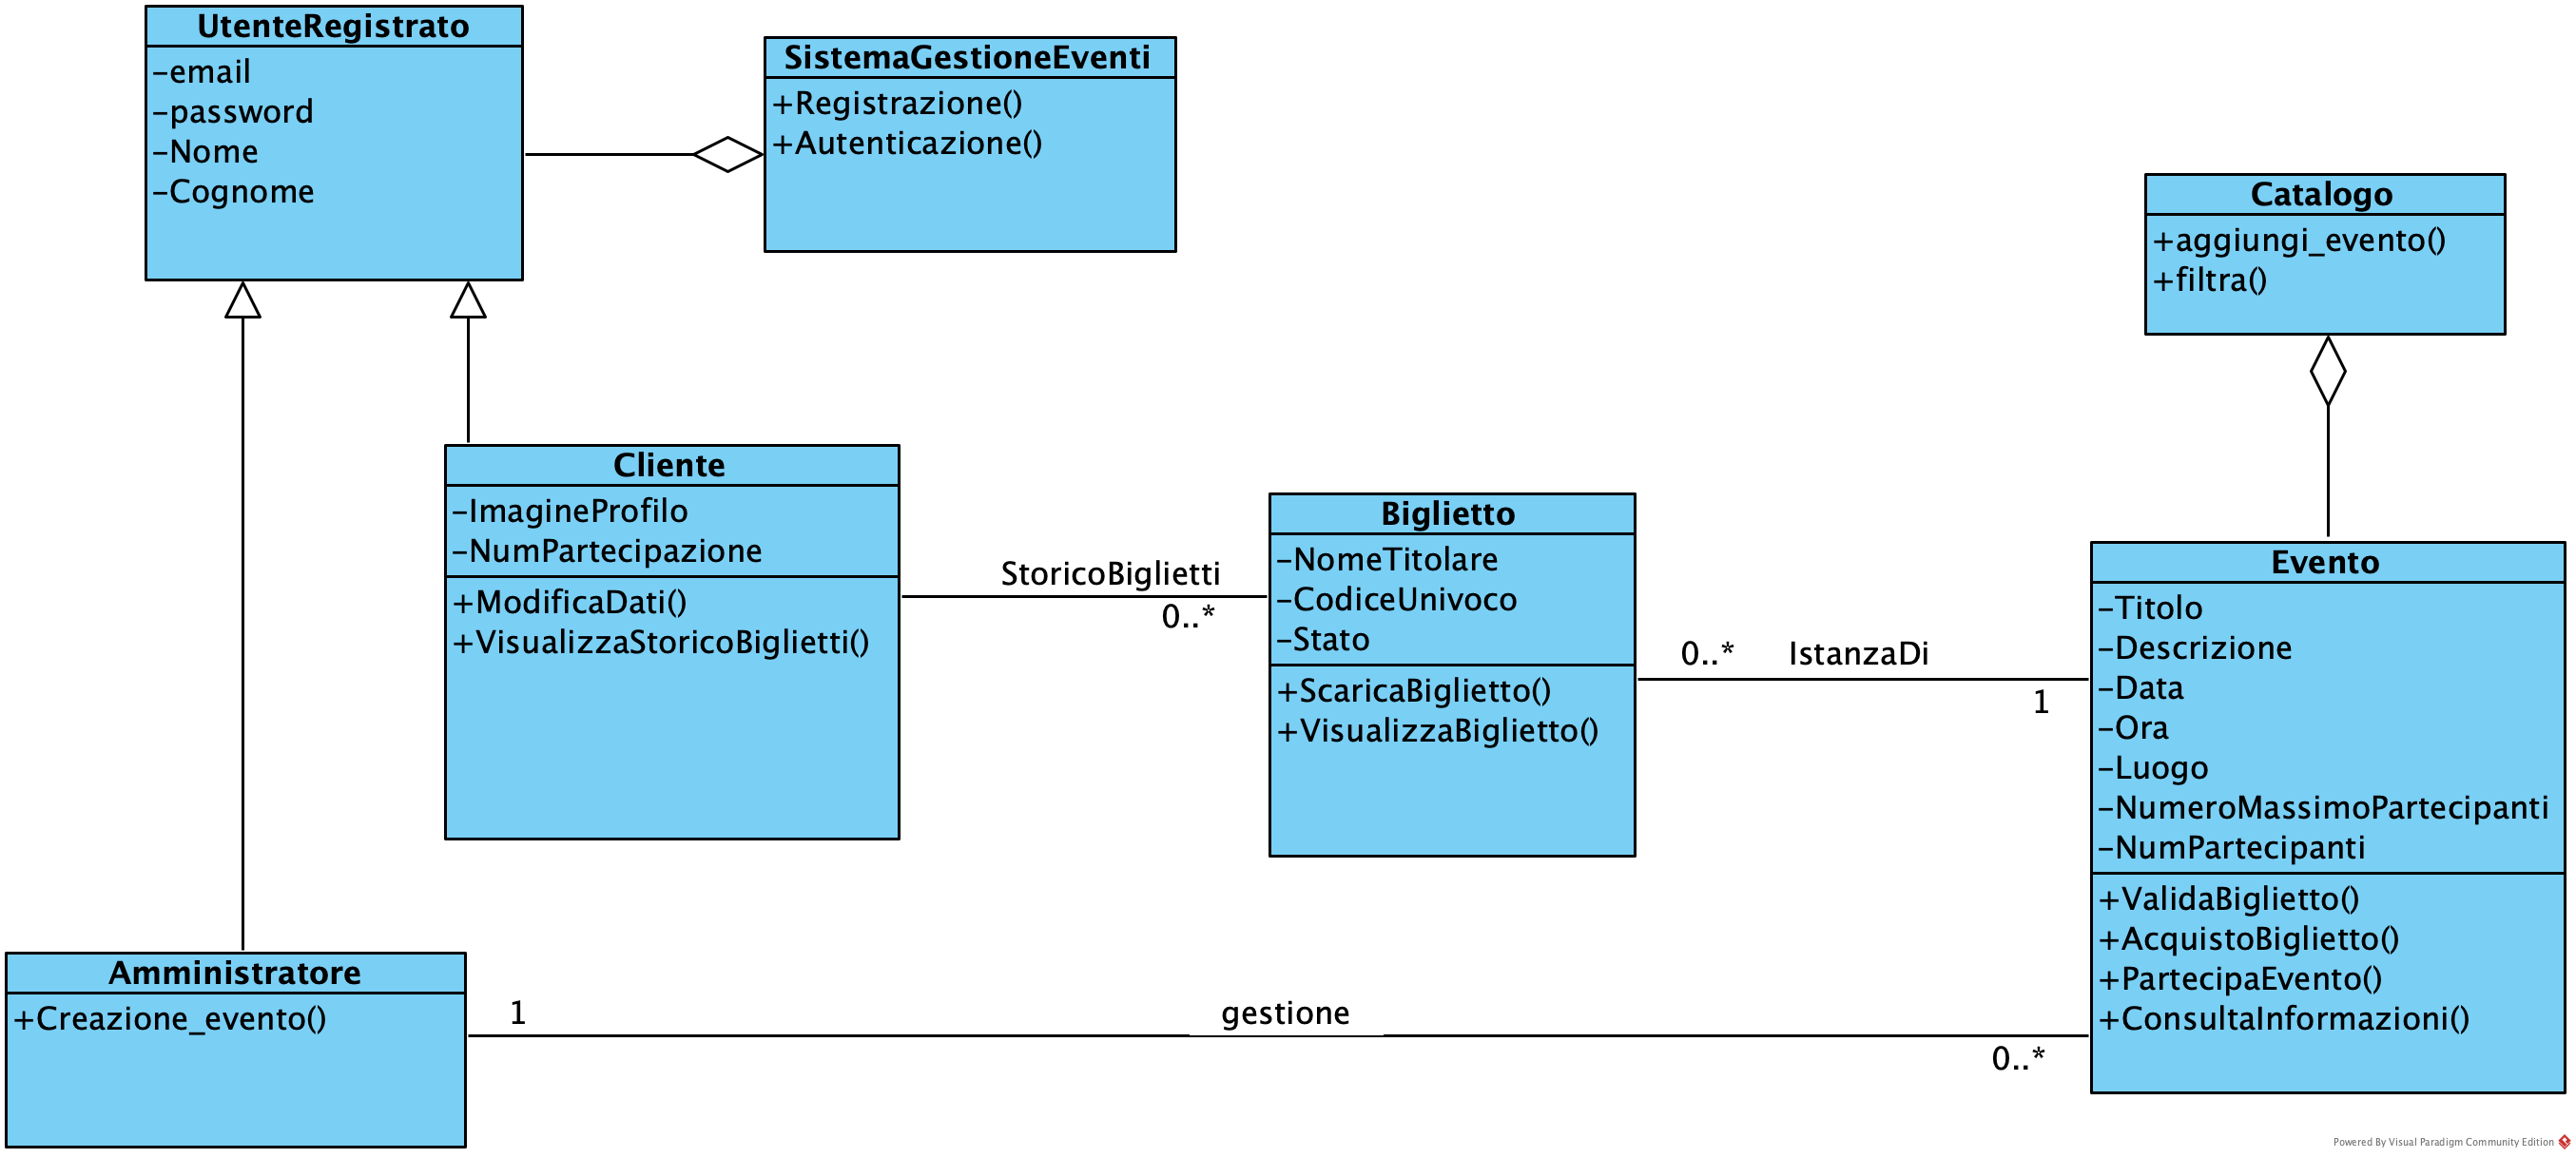
\includegraphics[width=0.8\linewidth]{assets/casid'uso/DiagramaDelleClassi.png}
	\caption{Diagramma delle classi di analisi}
\end{figure}


\begin{table}[h]
	\centering
	\begin{tblr}{
	  colspec = {X[0.6,c] X[0.6,c]},
	  width = 1\linewidth, 
	  hlines, vlines,
	  row{1} = {bg=gray!30, font=\bfseries}
	}
	RESPONSABILITÀ & CLASSE \\
	Registrazione & SistemaGestioneEventi \\
	Autenticazone & SistemagestioneEventi \\
	ModificaDati & Cliente \\
	VisualizzaStoricoBiglietti & Cliente \\
	CreazioneEvento & Amministratore \\
	ScaricaBiglietto & Biglietto \\
	VisualizzaBiglietto & Biglietto \\
	AcquistoBiglietto & Evento \\
	PartecipazioneEvento & Evento \\
	ConsultaInformazioni & Evento \\
	AggiungiEvento & Catalogo \\
	RicecaEvento & catalogo \\

	\end{tblr}
\end{table}

\begin{description}
	\item Registrazione e autenticazione sono responsabilità di \textbf{SistemaGestioneEventi} in quanto \textless\textless information expert \textgreater\textgreater{} di \textit{UtenteRegistrato}.
	
	\item ModificaDati e VisualizzaStoricoBiglietti sono responsabilità di \textbf{Cliente} in quanto agiscono su suoi attributi e classi ad esso associate.
	
	\item AcquistoBiglietto è una responsabilità di \textbf{Evento} in quanto \textless\textless creator \textgreater\textgreater{} di biglietti.
	
	\item PartecipazioneEvento è una responsabilità di \textbf{Evento} seguendo il pattern \textless\textless LOW COUPLING \textgreater\textgreater.
	
	\item AggiungiEvento è una responsabilità di \textbf{Catalogo} poiché, dopo la creazione, l’evento verrà aggiunto al catalogo.
	
	\item RicercaEvento è una responsabilità di \textbf{Catalogo} essendo il contenitore degli eventi.
	
	\item CreazioneEvento è una responsabilità di \textbf{Amministratore} essendo il \textless\textless creator \textgreater\textgreater{} di Eventi.
  \end{description}


\newpage

\section{Diagrammi di sequenza}

\subsection{Registrazione}

\begin{figure}[!ht]
	\centering
	La creazione del suddetto sequence diagram, sviluppato a partire dalla descrizione dello scenario del caso d’uso Accesso, ha fatto sorgere la necessità di definire un metodo, specifico per la classe SistemaGestioneEventi, verificaCredenziali(nomeUtente, password), privato, per consentire all’autonoleggio di verificare che le credenziali inserite dall’utente siano valide.
	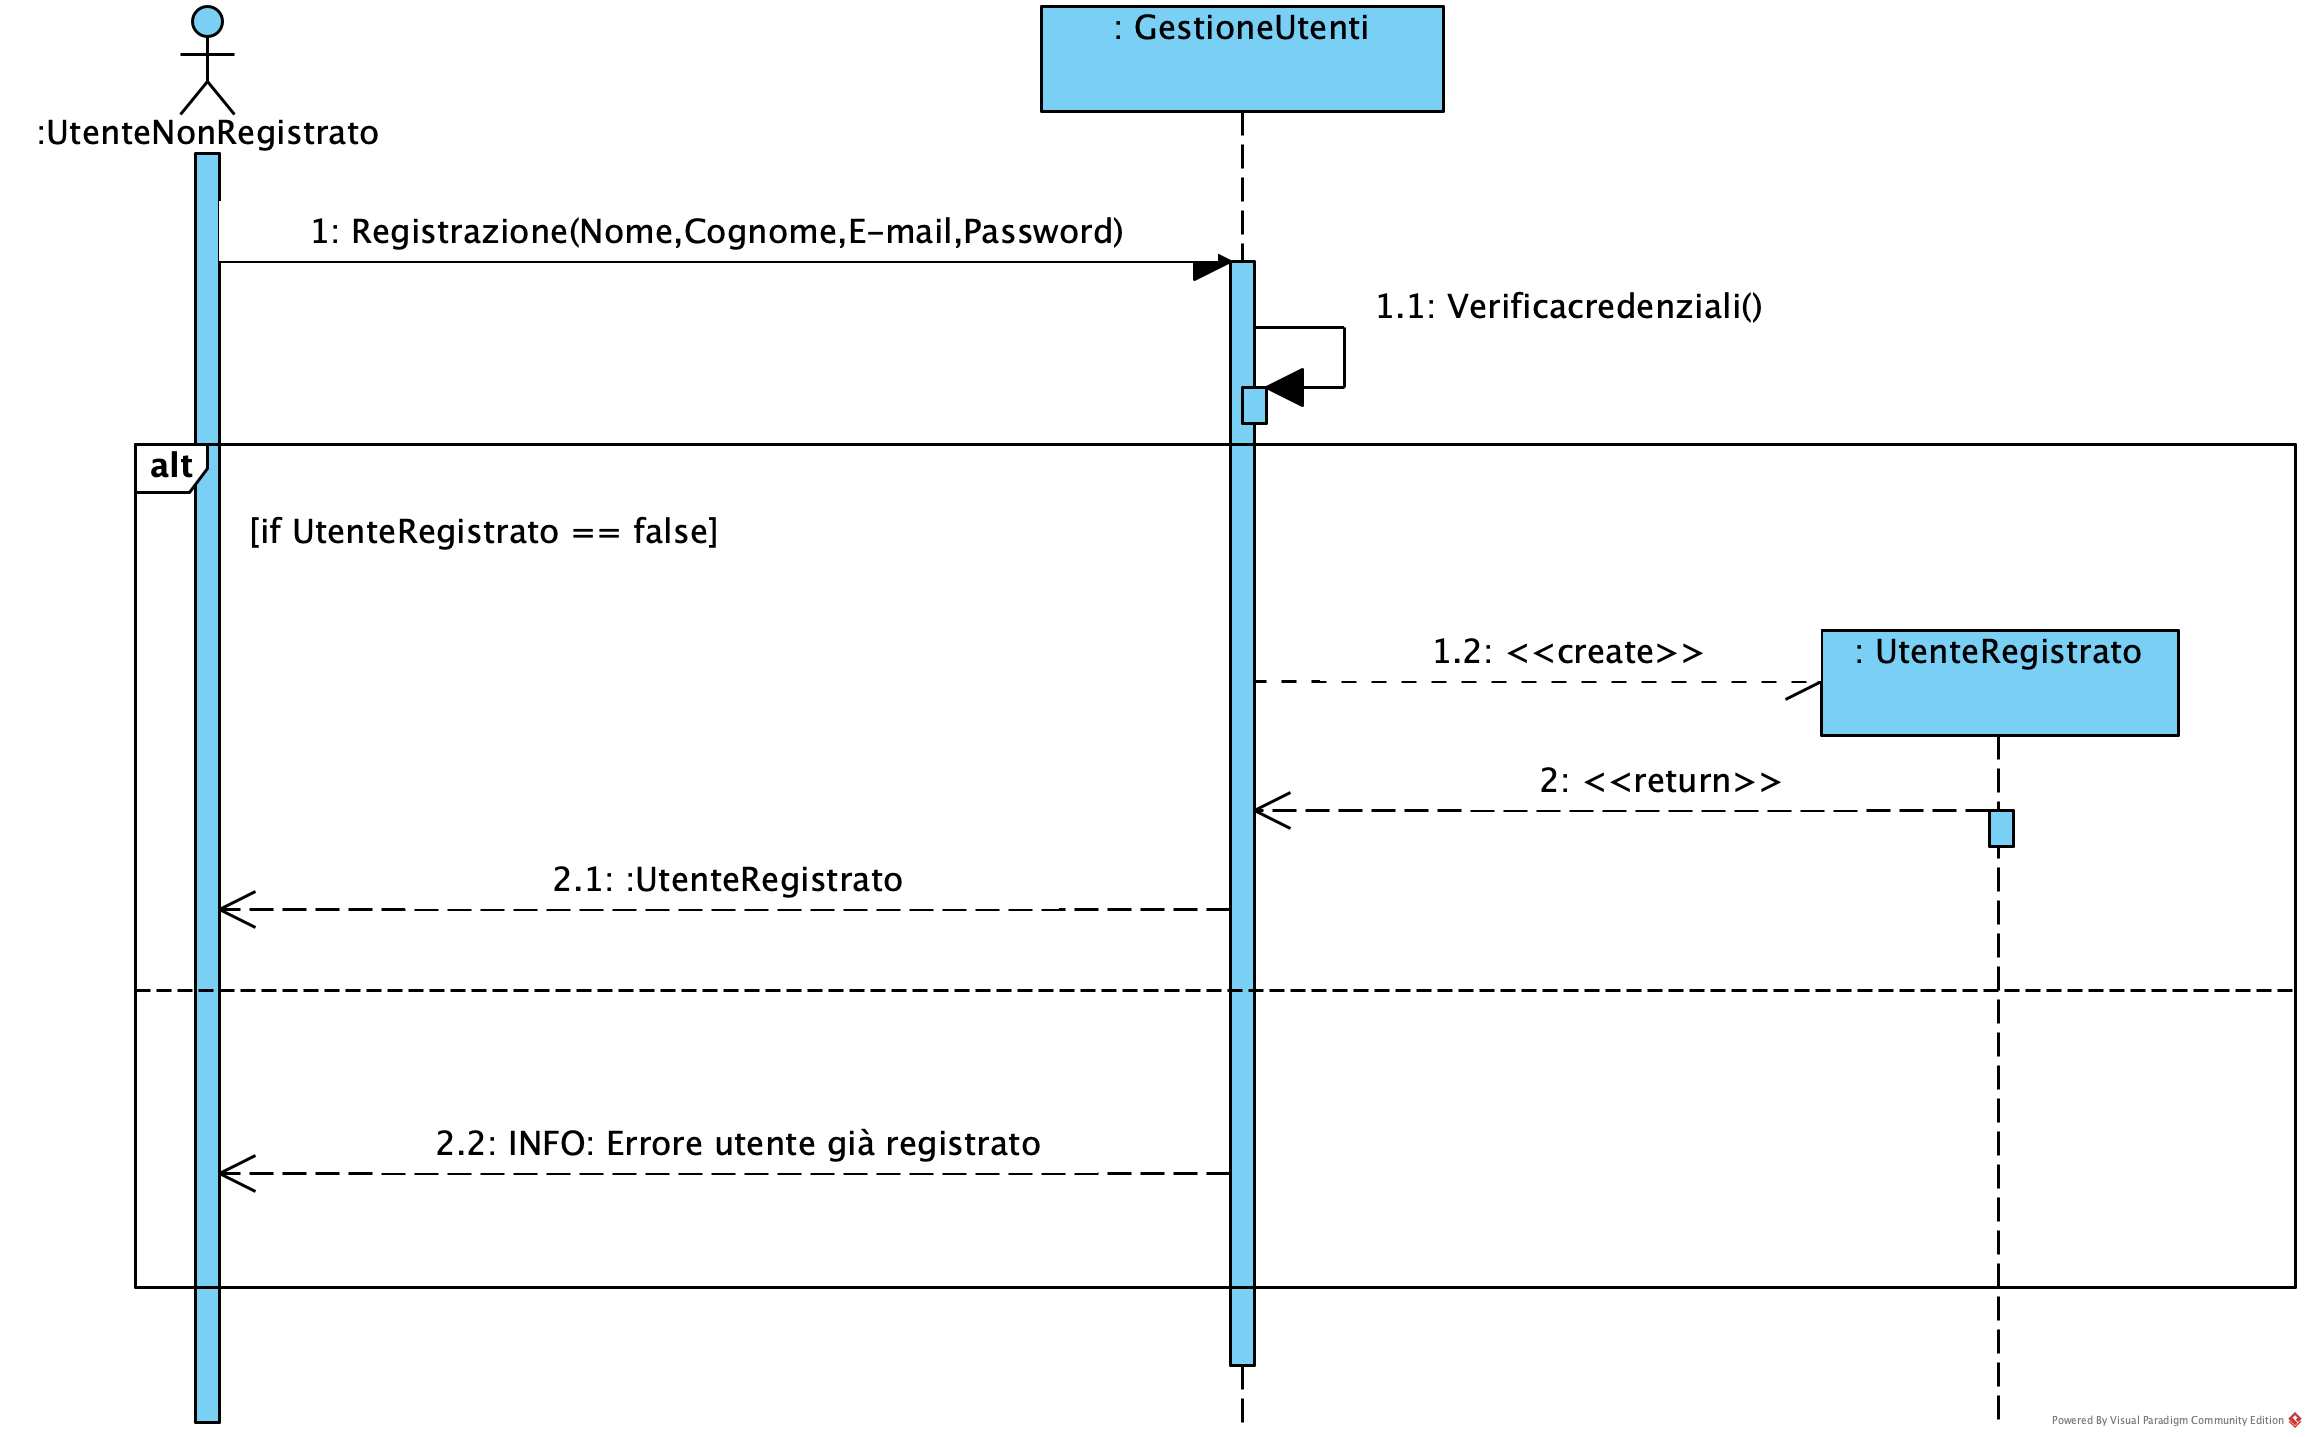
\includegraphics[width=0.8\linewidth]{assets/casid'uso/Registrazione.png}
\end{figure}


%autenticazione
%registrazione
%ConsultaCatalogoEventi
%AcquistoBiglietto
%PartecipazioneEvento
%RicercaEvento
%ConsultaInformazioniEvento
%pubblicaevento